\documentclass[a4paper]{article}
\usepackage[utf8]{inputenc}
\usepackage[russian,english]{babel}
\usepackage[T2A]{fontenc}
\usepackage[left=10mm, top=20mm, right=10mm, bottom=15mm, footskip=13mm]{geometry}
\usepackage{indentfirst}
\usepackage{amsmath,amssymb}
\usepackage{graphicx}
\usepackage[italicdiff]{physics}
\usepackage{float}
\usepackage{array}
\graphicspath{ {shema/} {graphic/} }
\usepackage{caption}
\captionsetup[figure]{name=Рисунок}
  
\title{Отчет по лабораторной работе 1.1.1

Измерение удельного сопротивления проволоки}

\author{Максим Осипов, Б03-504}
\date{10.09.2025}

\begin{document}
\maketitle

\section{Аннотация}

Работа посвящена измерению удельного сопротивления тонкой нихромовой проволоки. Электрическое сопротивление определяется двумя способами: через угол наклона графика зависимости напряжения от тока (с использованием аналоговых и цифровых вольтметров и амперметров) и с помощью моста постоянного тока. Диаметр и длина проволоки замеряются линейкой, штангенциркулем и микрометром. Центральное место в исследовании отводится детальному разбору погрешностей измерений, включая систематические и случайные.

\section{Теоретические сведения}

Удельное сопротивление материала проволоки круглого сечения изготовленной из однородного материала и имеющей постоянную толщину определяется по формуле:
\[ \rho = \frac{R_\text{пр}}{l}\frac{\pi d^2}{4}  \]
где $R_\text{пр}$ -сопротивление измеряемого отрезка проволоки, $l$ - его длина, $d$ - диаметр.
Поэтому измеряем длину, диаметр и электрическое сопротивление проволоки.\par
Диаметр у проволоки не постоянный поэтому нужно учесть случайную погрешность.
\begin{figure}[h!]
    \centering
    \includegraphics[width=0.5\textwidth]{shema}
    \caption{Схема для измерения сопротивления}
\end{figure}

\begin{figure}[h]
\centering
\includegraphics[width=0.4\linewidth]{изображение_2025-09-17_131240993.png}
\caption{Зависимость напряжения от силы тока для проводников разной длины}
\label{fig:voltage_current}
\end{figure}

По закону Ома: $R_\text{пр} = \frac{V_{a}}{I_{a}}$, где $V_{a}$ и $I_{a}$ - показания вольтметра и амперметра. Для измерения используем схему а) из учебника "Лабораторный практикум по общей физике т.1 Гладов" - рис.1, т.к. погрешность в измерениях там меньше чем в схеме б) (расчет будет в соответствующем параграфе).Получаем формулы для расчета: $R_\text{пр1} = \frac{V_{a}}{I_{a}} = R_\text{пр}\frac{R_{v}}{R_\text{пр} + R_{v}}$. Преобразовываем: $ R_\text{пр} = \frac{R_\text{пр1}}{1-(R_\text{пр1}/R_{v})} \approx R_\text{пр1}(1 + \frac{R_\text{пр1}}{R_{v}})$ (Используется приближение, т.к. сопротивление вольтметра $R_{v} \gg R_\text{пр},R_\text{пр1}$).\newline
График зависимости $V_{a}(I_{a})$ должен представлять прямую, угловой коэффициент которой и будет равен $R_{пр1}$.

\section{Оборудование и системные погрешности}

\begin{itemize}
  \item инека: $\sigma_\text{лин} = \pm0,5$ мм (о ене делени).
  \item Штангенциркуль: $\sigma_\text{штан} = \pm0,1$ мм (маркировка производителя).
  \item Микрометр:  $\sigma_\text{микр} = \pm0,01$ мм (маркировка производителя).
\end{itemize}  

\begin{table}[htbp]
\centering
\caption{Характеристики приборов}
\begin{tabular}{|c|c|c|}
\hline
 & Амперметр & Вольтметр \\
\hline
система прибора & электромагнитная & цифорвая \\
\hline
класс точности & 0,5 & \\
\hline
предел измерений & 0,75А & \\
\hline
число делений шкалы & 150 & \\
\hline
цена деления & 0,5мА/дел & \\
\hline
чувствительность & 200дел/A & \\
\hline
внутреннее сопротивление & пренебрежимо мало & 10 МОм\\
\hline
\end{tabular}
\end{table}

\section{Результаты измерений и обработка данных}
\subsection{Измерение диаметра проволоки}
\begin{center}
    \begin{tabular}{|c | c | c | c | c | c | c | c | c | c | c |} 
     \hline
      & 1 & 2 & 3& 4& 5& 6 & 7 & 8 & 9 & 10 \\
    \hline
     $d_\text{штанг}$, мм & 0,4 & 0,4 & 0,4 & 0,4 & 0,4 & 0,4 & 0,4 & 0,4 & 0,4 & 0,4  \\ 
     \hline
     $d_\text{микр}$, мм & 0,35 & 0,34 & 0,36 & 0,36 & 0,34 & 0,35 & 0,37 & 0,33 & 0,35 & 0,36 \\
     \hline
    \end{tabular} 
\end{center}

Погрешности: 

\begin{itemize}
\item Среднее значение: $\langle d \rangle = \frac{1}{n}\sum\limits_{i=1}^n d_{i} = 0.348$ мм. 
\item Стандартное отклонение: $\sigma_\text{d} = \sqrt{\frac{1}{n}\sum\limits_{i=1}^n(d_{i} - \langle d \rangle)^2} =0.001$ мм.
\item Стандартная погрешность опыта: $\sigma_\text{ср} = \frac{\sigma_\text{d}}{\sqrt{n}} =0.003$   мм.
\item Полная погрешность: $\sigma_\text{полн} = \sqrt{\sigma_\text{ср}^2 + \sigma_\text{микр}^2} =0.005$  мм.
\end{itemize}

\begin{table}[H]
\centering
\caption{ВАХ проволоки}
\large
\begin{tabular}{|>{\centering\arraybackslash}m{1.8cm}|>{\centering\arraybackslash}m{1.8cm}||>{\centering\arraybackslash}m{1.8cm}|>{\centering\arraybackslash}m{1.8cm}||>{\centering\arraybackslash}m{1.8cm}|>{\centering\arraybackslash}m{1.8cm}|}
\hline
\multicolumn{2}{|c||}{\textbf{$l = 20$ см}} & \multicolumn{2}{c||}{\textbf{$l = 30$ см}} & \multicolumn{2}{c|}{\textbf{$l = 50$ см}} \\ \hline
$U$, мВ & $I$, мА & $U$, мВ & $I$, мА & $U$, мВ & $I$, мА \\ \hline
141     & 130   & 220     & 130   & 322     & 110     \\ \hline
166     & 140   & 241     & 150   & 341     & 120     \\ \hline
181     & 160   & 288     & 170   & 386     & 140     \\ \hline
216     & 190   & 335     & 200   & 426     & 150     \\ \hline
232     & 210   & 395     & 280   & 555     & 200     \\ \hline
266     & 230   & 486     & 290   & 630     & 220     \\ \hline
301     & 260   & 626     & 370   & 720     & 260     \\ \hline
368     & 320   & 680     & 400   & 774     & 310     \\ \hline
470     & 360   & 873     & 510   & 813     & 400     \\ \hline
681     & 590   & 916     & 660   & 866     & 470     \\ \hline

\end{tabular}
\end{table}

\begin{figure}[h]
\centering
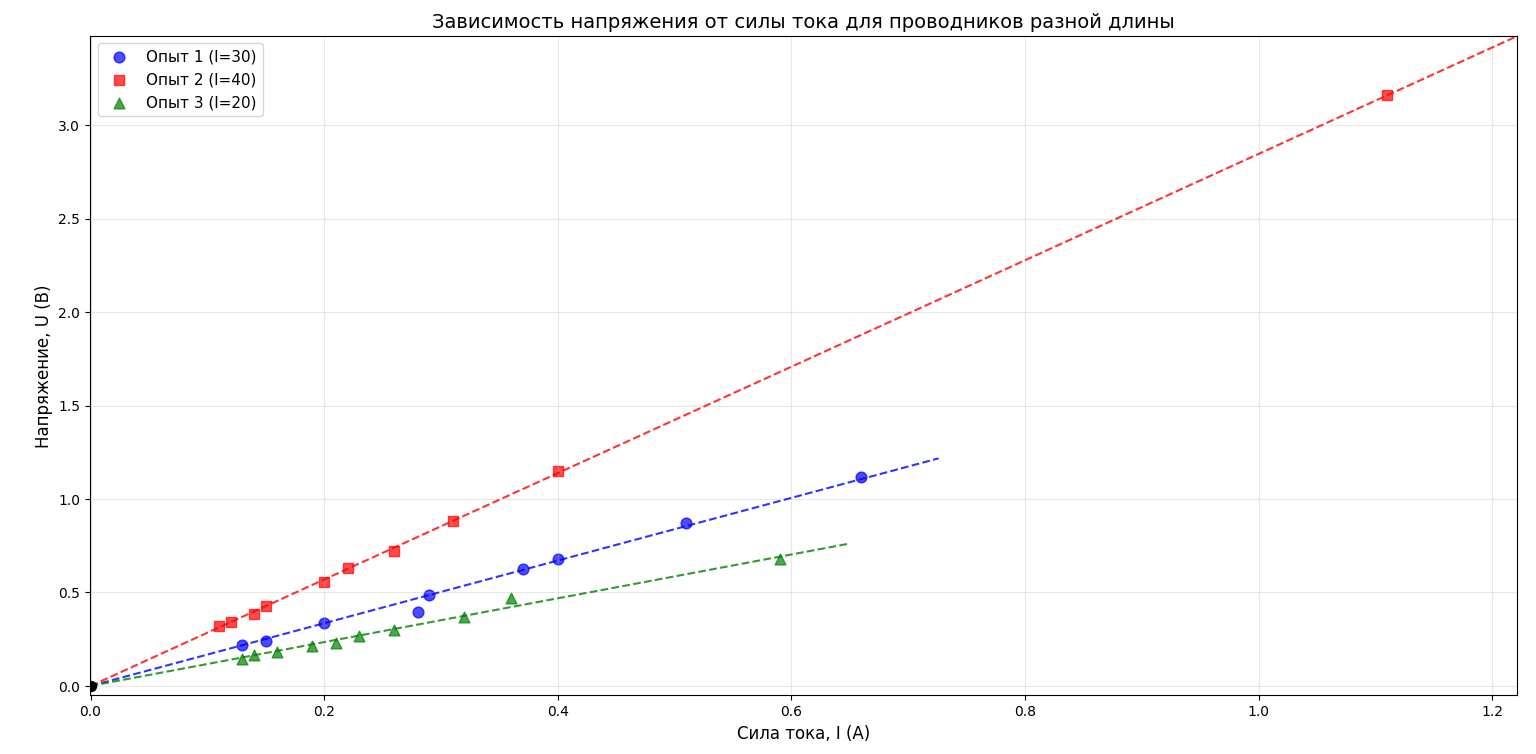
\includegraphics[width=0.8\linewidth]{ВАХ.png}
\caption{Зависимость напряжения от силы тока для проводников разной длины}
\label{fig:voltage_current}
\end{figure}



Результаты исследований зависимостей показаний вольтметра $V_{a}$  от показаний амперметра $I_{a}$ представлены графике ВАХ.
С помощью метода наименьших квадратов были построены аппроксимирующие прямые $V_{B} = \langle R \rangle I_{A}$ по формуле: \[ \langle R \rangle = \frac{\langle VI \rangle}{\langle I^2 \rangle}\]\par
Погрешность угла наклона в аппроксимации(т.е. погрешность $\langle R \rangle$) найдем как косвенную погрешность наименьших квадратов по формуле: $\sigma_{R\text{случ}} = \sqrt{\frac{1}{n-1}(\frac{\langle V^2 \rangle}{\langle I^2 \rangle}-\langle R \rangle^2)}$.\par
Систематическую погрешность найдем как частные производные за значения выбрав наибольшие измерения: \[ \sigma_{R\text{сист}} = R \sqrt{\left(  \frac{\sigma_{V}}{Vmax}\right)^2 + \left(\frac{\sigma_{I}}{Imax}\right)^2}  \] \par
Полную погрешность вычислим по формуле: \[\sigma_{R\text{полн}} = \sqrt{\left( \sigma_{R\text{случ}}\right)^2 + \left( \sigma_{R\text{сист}}\right)^2} \] \par

% Исправленная таблица - убрано [H] и добавлено \centering
\begin{table}[htbp] % Используем htbp для лучшего позиционирования
\centering
\caption{Сопротивления}
\begin{tabular}{|c|c|c|c|c|c|c|}
\hline
$l$, см & $R_{\mbox{\tiny{ср}}}$, Ом & $\sigma_R^{\mbox{\tiny{сл}}}$, Ом & $\sigma_R^{\mbox{\tiny{сист}}}$, Ом & $R_{\mbox{\tiny{пр}}}$, Ом & $\sigma_R$, Ом & $R_{\mbox{\tiny{мост}}}$, Ом \\ \hline
20      & 2,34                       & 0,04                              & 0,01                                & 2,34                        & 0,05           & 2,134                       \\ \hline
30      & 3,15                       & 0,02                              & 0,02                                & 3,15                       & 0,03           & 3,150                       \\ \hline
50      & 5,09                          & 0,14                              & 0,01                                & 5,09                        & 0,14           & 5,196                       \\ \hline
\end{tabular}
\end{table}
 Поправка $R_{\mbox{\tiny{ср}}}/R_V \ll 1$, поэтому ее погрешность можно не учитывать.

 \item Согласно формуле (1) зависимость $R_{\mbox{\tiny{пр}}}(l)$ должна быть линейной, поэтому
    применим МНК для анализа данных, представленных в таблице 3. Погрешность найдем как
    \[
        \frac{\sigma_{\rho}}{\rho} = \sqrt{\left(\frac{\sigma_R}{R}\right)^2 +
        \left(\frac{2\sigma_d}{d}\right)^2}
    \]







Результаты для каждой из длин представлены в таблице \ref{удсопрот}

\begin{table}[h]
\centering
\caption{Результаты измерения $\rho$ для каждой из длин проволок}
\begin{tabular}{|c|c|c|}
\hline 
$l$, см & $\rho$, $10^{-6}$ Ом $\cdot$м &$\sigma_{\rho}$, $10^{-8}$Ом$\cdot$м \\ 
\hline 
20 & 1.06 & 5,19 \\ 
\hline 
30 & 1.06 & 3,29 \\ 
\hline 
50 & 1.08 & 6,34 \\ 
\hline 
\end{tabular} 
\label{удсопрот}
\end{table}

Окончательно $\rho = (1.10 \pm 0.04)\cdot 10^{-6}$ Ом$\cdot$м.

\section{Вывод}
В ходе эксперимента было определено удельное сопротивление нихромовой проволоки с точностью порядка  {5\%} . Полученное значение ρитог = (1,07 ± 0,052)·10⁻⁶ Ом·м находится в пределах табличного диапазона для нихромового сплава, который составляет от 0,97 до 1,14·10⁻⁶ Ом·м.

Особое внимание в работе было уделено анализу погрешностей. Сравнительный анализ показал, что случайная погрешность измерений на порядок меньше систематической, что свидетельствует о преобладающем влиянии инструментальной погрешности измерительного оборудования. Наибольший вклад в общую погрешность результата внесла погрешность измерений микрометром, которая и оказалась определяющей для итоговой погрешности определения удельного сопротивления.



\end{document}